\section{Sum-Product Networks}

\begin{frame}{Sum-Product Networks}
\begin{itemize}
    \item Sum-product networks (SPNs)\footnote{\scriptsize H. Poon \& P. Domingos: Sum-product networks: A new deep architecture. In UAI, 2011.} are a sub-class of so-called tractable probabilistic models or probabilistic circuits\footnote{\scriptsize Van den Broeck et al.: Tractable probabilistic models: Representations, algorithms, learning and applications. Tutorial at UAI, 2019.}, that admit tractable probabilistic inference.
    \item A class of queries $Q$ on a class of models $M$ is tractable, iff for any query $q \in Q$ and model $m \in M$ the computational complexity is at most polynomial.
    \item SPNs admit many probabilistic inference tasks, such as marginalisation, in linear time in their representation size.
\end{itemize}
\end{frame}

\begin{frame}{Probabilistic Inference}
\begin{table}
\centering
\begin{tabular}{lllll}
             & GANs & VAEs & Flows & SPNs  \\
Sampling     & Y    & Y    & Y     & Y      \\
Density      & N    & N/Y  & Y     & Y      \\
Marginals    & N    & N    & ?     & Y      \\
Conditionals & N    & N    & ?     & Y      \\
Moments      & N    & N    & ?     & Y      \\
MAP          & N    & N    & ?     & N/Y
\end{tabular}
\caption{\scriptsize Robert Peharz, Sum-Product Networks and Deep Learning: A Love Marriage. Talk at ICML, 2019.}
\end{table}
\end{frame}

\begin{frame}{What is a Sum-Product Network?}
\begin{itemize}
  \item Let $\X = \{X_1, \dots, X_D\}$ be set of $D$ random variables.
  \item A Probabilistic Circuit (PC) is a tuple $\SPN = (\graph, \scope, \tp)$, where
  \begin{itemize}
    \item $\graph$ is a computational graph.
    \item $\scope$ is a so-called scope function.
    \item $\w$ denotes the set of parameters, e.g. sum-weights and leaf node parameters.
  \end{itemize}
  \item A Sum-Product Network (SPN) is a \emph{smooth} and \emph{decomposable} PC.
\end{itemize}
\end{frame}

\begin{frame}{Computational Graph $\graph$}
 $\graph$ is a rooted connected directed acyclic graph (DAG), containing: sum ($\SumNode$), product ($\ProductNode$) and leaf nodes ($\Leaf$).

\begin{figure}
  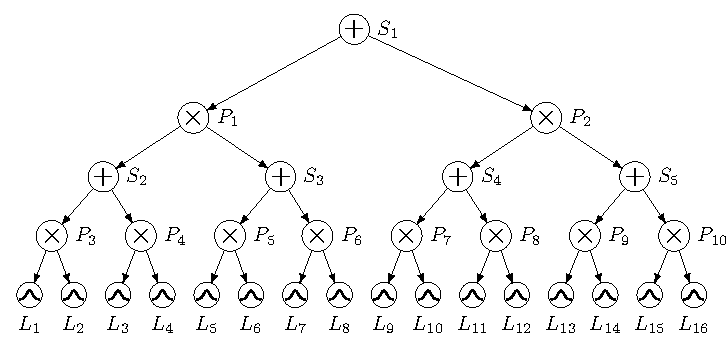
\includegraphics[width=\textwidth]{computation_graph}
  \caption{Example of a tree-shaped computational graph.}
\end{figure}
\end{frame}

\begin{frame}{Leaves $\Leaf$ in $\graph$}
    Leaf/input nodes are arbitrary (tractable) distributions, e.g.~Gaussian, Multinomial, variational autoencoder.\\[1em]

\tikzstyle{vertex}=[inner sep=0.01cm, circle, draw]
\begin{columns}
\begin{column}{.2\linewidth}
\end{column}
\begin{column}{.2\linewidth}
\begin{tikzpicture} [scale=0.5, auto,>=latex,transform shape]
   \node[draw=none](v01) at (1, 1.5) {};
   \node[draw=none](v02) at (-1, 1.5) {};
   \node[vertex](v1) at (0, 0) {\usebox{\genericfiltLarge}};
   \draw [->] (v01) -- (v1);
   \draw [->] (v02) -- (v1);
\end{tikzpicture}
\end{column}
\begin{column}{.4\linewidth}
$\Leaf(x) = p(x \cbar \tp_\Leaf)$
\end{column}
\begin{column}{.2\linewidth}
\end{column}
\end{columns}

\centering
\begin{figure}
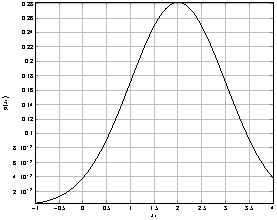
\includegraphics{leaf_distribution}
\end{figure}
\end{frame}

\begin{frame}{Product Nodes $\ProductNode$ in $\graph$}
Product nodes encode independence assumptions between sets of random variables.\\[1em]

 \tikzstyle{vertex}=[inner sep=0.01cm, circle, draw]
\begin{columns}
\begin{column}{.2\linewidth}
\end{column}
\begin{column}{.2\linewidth}
\begin{tikzpicture} [scale=0.5, auto,>=latex,transform shape]
   \node[draw=none](v01) at (1, 1.5) {};
   \node[draw=none](v02) at (-1, 1.5) {};
   \node[draw=none](v21) at (1, -1.5) {};
   \node[draw=none](v22) at (-1, -1.5) {};
   \node[vertex](v1) at (0, 0) {\huge$\bm\times$};
   \draw [->] (v01) -- (v1);
   \draw [->] (v02) -- (v1);
   \draw [->] (v1) -- (v21);
   \draw [->] (v1) -- (v22);
\end{tikzpicture}
\end{column}
\begin{column}{.4\linewidth}
$\ProductNode(x)  = \prod\limits_{\Child \in \ch(\ProductNode)} \Child(x)$
\end{column}
\begin{column}{.2\linewidth}
\end{column}
\end{columns}

\centering
\begin{figure}
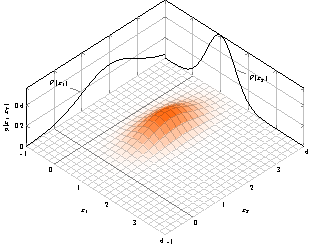
\includegraphics{product_distribution}
\end{figure}
\end{frame}

\begin{frame}{Sum Nodes $\SumNode$ in $\graph$}
    Sum nodes\footnote{\scriptsize $\sum_{\Child \in \ch(\SumNode)} w_{\SumNode,\Child} = 1$ and $\w_{\SumNode, \Child} \geq 0$.} replace independence with conditional independence within the network.\\[1em]

\tikzstyle{vertex}=[inner sep=0.01cm, circle, draw]
\begin{columns}
\begin{column}{.2\linewidth}
\end{column}
\begin{column}{.2\linewidth}
\begin{tikzpicture} [scale=0.5, auto,>=latex,transform shape]
   \node[draw=none](v01) at (1, 1.5) {};
   \node[draw=none](v02) at (-1, 1.5) {};
   \node[draw=none](v21) at (1, -1.5) {};
   \node[draw=none](v22) at (-1, -1.5) {};
   \node[vertex](v1) at (0, 0) {\huge$\bm+$};
   \draw [->] (v01) -- (v1);
   \draw [->] (v02) -- (v1);
   \draw [->] (v1) -- (v21);
   \draw [->] (v1) -- (v22);
\end{tikzpicture}
\end{column}
\begin{column}{.4\linewidth}
$\SumNode(x)  = \sum\limits_{\Child \in \ch(\ProductNode)}  \w_{\SumNode, \Child}\Child(x)$
\end{column}
\begin{column}{.2\linewidth}
\end{column}
\end{columns}

\centering
\begin{figure}
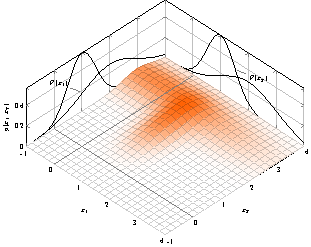
\includegraphics{sum_distribution}
\end{figure}
\end{frame}

\begin{frame}{Scope Function $\scope$}
$\scope$ is a function assigning each node $\Node$ in a sub-set of $\X$,\footnote{\scriptsize This sub-set is often referred to as the scope of a node.} and has to fulfil the following properties:
\begin{defbox}
\begin{enumerate}
\item If $\Node$ is the root node, then $\scope(\Node) = \X$.
\item If $\Node$ is a sum or product, then $\scope(\Node) = \bigcup_{\Node' \in \ch(\Node)} \scope(\Node')$.
\item For each $\SumNode \in \SumNodes$ we have $\forall \Node, \Node' \in \ch(\SumNode)\colon \scope(\Node) = \scope(\Node')$ (\emph{smoothness})
\item For each $\ProductNode \in \ProductNodes$ we have $\forall \Node, \Node' \in \ch(\ProductNode)\colon \scope(\Node) \cap \scope(\Node') = \emptyset$ (\emph{decomposability}).
\end{enumerate}
\end{defbox}
\end{frame}

\frame{
\begin{center}Example SPN $\SPN = (\graph, \scope, \w, \tp)$\end{center}
\begin{figure}
  \centering{
    \includestandalone[width=0.9\textwidth]{SPN}
    }
\end{figure}
After applying a scope function $\scope$  on $\graph$ we obtain the SPN. Most structure learners learn both in an entangled way.

\small Note that we define $\Leaf(x):=1$ for every $x$ if and only if $\scope(\Leaf) = \emptyset$.
}
